\subsection{Примеры неустойчивых решений уравнения теплопроводности}
\vspace{1em}

\newtheorem{exmp}{Пример}

\begin{exmp}
\end{exmp}

В качестве начальных условий возмем $u_0 = sin(\pi x)$. Продемонстрируем 
неустойчивость нулевого решения при $\alpha = \pi^2 + 0.1$.

\begin{figure}[H]
    \centering
        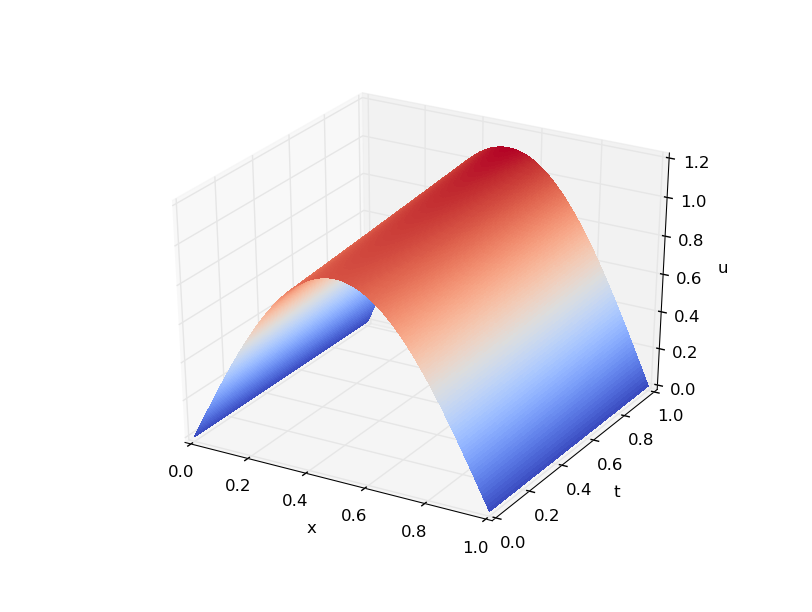
\includegraphics[width=3.5in]{par_ex_pi01}
        \caption{Без управления}
        \label{fig:test1}
\end{figure}

\begin{exmp}
\end{exmp}

Пусть $u(x, 0) = x(1 - x)$ - начальное условие . Заведомо выберем параметр 
$\alpha = \pi^2 + 3$ большим. 

\begin{figure}[H]
    \centering
        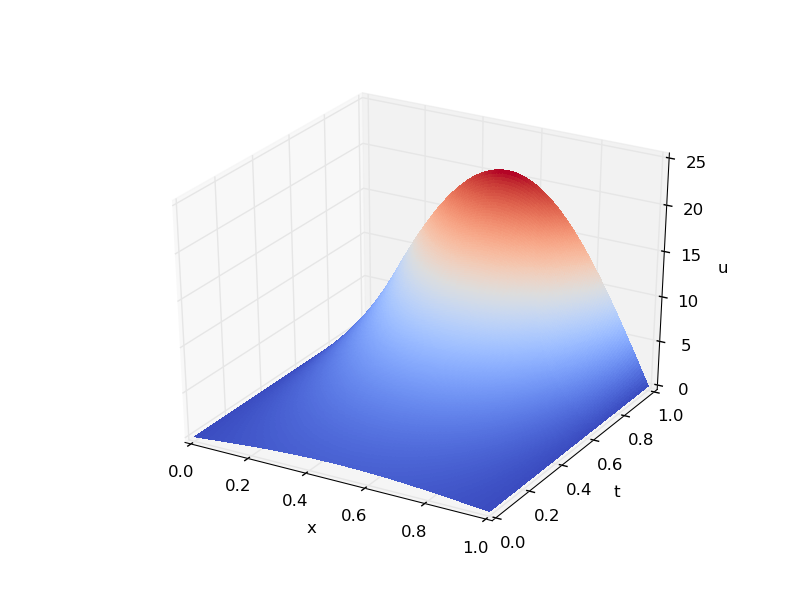
\includegraphics[width=3.5in]{par_ex_pi3}
        \caption{Без управления}
        \label{fig:test1}
\end{figure}

